\documentclass[a4paper, 11pt]{article}
\usepackage[top=3cm, bottom=3cm, left = 2cm, right = 2cm]{geometry} 
\geometry{a4paper} 
\usepackage[utf8]{inputenc}
\usepackage{textcomp}
\usepackage[italian]{babel}
\usepackage{graphicx} 
\usepackage{guit}
\usepackage{amsmath,amssymb}  
\usepackage{filecontents}
\usepackage{bm}  
\usepackage[pdftex,bookmarks,colorlinks,breaklinks]{hyperref}  
\hypersetup{linkcolor=black,citecolor=black,filecolor=black,urlcolor=black} 
\usepackage{memhfixc} 
\graphicspath{ {images/} }
\usepackage{pdfsync}  
\usepackage{fancyhdr}
 \usepackage[
    backend=biber,
    style=ieee,
  ]{biblatex}\graphicspath{ {images/} }
\pagestyle{fancy}


\addbibresource{biblio.bib}

\author{Martina Salvati}
\title{ANALISI CONSUMI ENERGETICI TRAMITE POWERAPI}
\date{\today} % Sets date for date compiled

\begin{document}
\maketitle
\tableofcontents

\section{Introduzione}

In questo report discuto i risultati ottenuto dall'utilizzo di SmartWatts (powerApi).

\pagebreak

\section{Power meter Architecture}
Un misuratore di potenza è un insieme di due componenti, un sensore e una formula, utilizzati per produrre una stima del consumo energetico di un software monitorato.

Il sensore raccoglie i dati grezzi correlati al consumo energetico del software. La formula è un modulo computazionale che utilizza i dati raccolti per determinare il consumo energetico. Entrambi sono collegati da un database che viene utilizzato per trasferire le informazioni. L'architettura globale di un misuratore di potenza è rappresentata di seguito.

\begin{figure}[h]
\centering
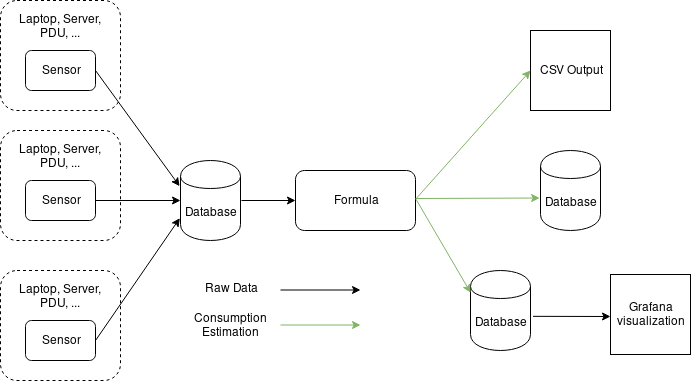
\includegraphics[scale=0.65]{powerAPI_archi}
\centering
\end{figure}
\pagebreak
\subsubsection{Sensore}
Un sensore è un software indipendente che raccoglie dati grezzi correlati al consumo energetico del software monitorato.

I dati vengono raccolti interrogando la macchina dell'hardware che ospita il software monitorato. Il sensore deve essere eseguito sulla stessa macchina del software monitorato. I dati vengono raccolti per tutta la durata del software. Per questo motivo il sensore deve funzionare in parallelo.

I dati raccolti vengono archiviati in un database esterno per rendere i dati disponibili alla formula. Questo database può essere ospitato su un'altra macchina.
\subsubsection{Formula}
Una formula è un software indipendente che calcola una stima del consumo energetico del software monitorato dai dati raccolti dal sensore. (es: Smartwatts).
Una formula comunica con il sensore tramite un database (es. MongoDB). Il sensore scrive i dati raccolti nel database e la formula li legge in seguito.
Ci sono due modalità di connessione:
\begin{itemize}
\item modalità flusso in cui la formula legge i dati dal sensore mentre vengono prodotti
\item   modalità post mortem che analizza i dati già raccolti dal sensore in una fase di monitoraggio passata.
\end{itemize}
  

\subsection{SmartWatts}
SmartWatts è un misuratore di potenza definito dal software basato sul toolkit PowerAPI. SmartWatts è un software configurabile in grado di stimare il consumo energetico del software in tempo reale. 

Smartwatt si basa su due interfacce di sistema ampiamente disponibili: - RAPL per raccogliere le misurazioni di base per la potenza della CPU e della DRAM consumi.
- HWPC, l'interfaccia degli eventi perf di Linux. per acquisire gli eventi Hardware Performance Counters. HWPC viene utilizzata per stimare il consumo energetico per contenitore da modelli di alimentazione specifici delle risorse, che vengono adattati in fase di esecuzione.


Gli SmartWatt devono ricevere diversi parametri forniti da hwpc-sensor.
\begin{itemize}
\item   \ The Running Average Power Limit (RAPL)
\item   \ TSC
\item  \ APERF
\item   \ MPERF
\item    \ CPU CLK THREAD UNHALTED:REF P 
\item   \ CPU CLK THREAD UNHALTED:THREAD P 
\item   \ LLC MISSES 
\item   \ INSTRUCTIONS RETIRED 
\end{itemize}


In particolare, il raggiungimento di una pianificazione ottimale dei container richiede l'implementazione di misuratori di potenza software-defined per andare oltre la granularità dei sensori di monitoraggio dell'alimentazione hardware, come le unità di distribuzione dell'alimentazione (PDU) o il limite di potenza media in esecuzione (RAPL) di Intel, per fornire energia stime delle attività alla granularità dei contenitori software. 

Tuttavia, la definizione dei modelli di alimentazione sottostanti che stimano il consumo energetico rimane un processo lungo e fragile che è strettamente collegato alla macchina host.
 
Per superare queste limitazioni, questo documento introduce \textbf{SmartWatts}: un sistema leggero di monitoraggio dell'alimentazione che adotta la calibrazione online per regolare i modelli di potenza di CPU e DRAM per massimizzare l'accuratezza delle stime di potenza di runtime dei container.
 
A differenza delle tecniche all'avanguardia, SmartWatts non richiede alcuna fase di formazione a priori o attrezzatura hardware per configurare i modelli di potenza e può quindi essere implementato su un'ampia gamma di macchine, comprese le ultime ottimizzazioni di potenza, senza alcun costo.

\begin{figure}[h]
\centering
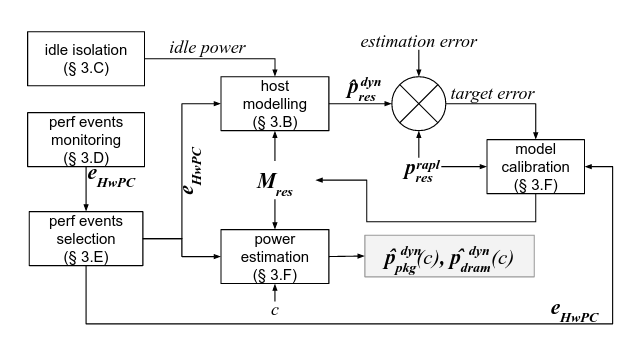
\includegraphics[scale=0.65]{smartwatts}
\centering
\end{figure}


Smartwatts gestisce in runtime una serie di auto-modelli a potenza calibrata ì per ciascuna potenza monitorabile
risorse (ad es. CPU, DRAM). Questi modelli di potenza sono
quindi utilizzato da Smartwatts per stimare il consumo di energia dell'host e dei container ospitati sull'host. 

Per catturare meglio il consumo energetico dinamico del host, SMARTWATTS ha bisogno di isolare il suo consumo statico.

SMARTWATTS effettua le stime del consumo energetico dell'host da un insieme di input che si riferiscono a eventi HWPC, che sono selezionati in tempo di esecuzione.

Questo design assicura che SMARTWATTS continui a regolare i
modelli di potenza per massimizzare l'accuratezza della stima della potenza.

L'isolamento del consumo di energia statica di un nodo è un
problema impegnativo in quanto richiede di raggiungere uno stato di quiete per catturare il consumo energetico dell'host a riposo.

\subsubsection{Implementazione}
Il sensore consiste in un software leggero distribuito su tutti i nodi che devono essere monitorati.

\subsubsection{Stime}
Le stime della potenza vengono fornite per ogni nodo e per i Cgroup di interesse. Gli scopi di questi Cgroup possono riflettere l'attività del kernel dei nodi e sistema, nonché qualsiasi lavoro o servizio in esecuzione nel monitorato ambiente. Queste stime di potenza possono quindi essere aggregate per proprietario, identificatore di servizio o qualsiasi altra chiave, a seconda di casi d'uso. Possono anche essere aggregati lungo il tempo da segnalare sull'impronta energetica di un dato sistema software.
\subsection{Analisi consumi}

\subsubsection{Analisi energia globale}
\begin{flushleft}
Per la rappresentazione di questo grafico viene fatta la somma ogni secondo della potenza istantanea.
\end{flushleft}
\begin{figure}[h]
\caption{CONSUMI ENERGETICI GLOBALI}
\centering
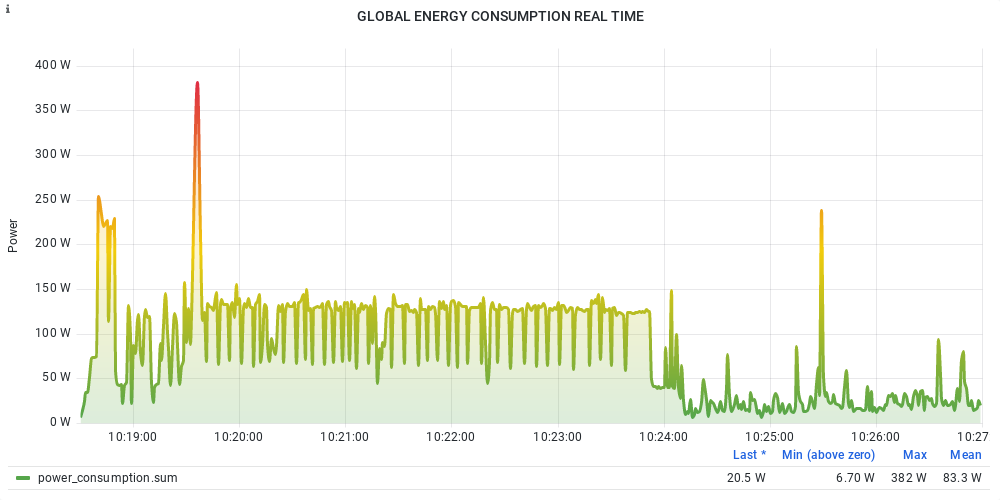
\includegraphics[scale=0.4]{image2}
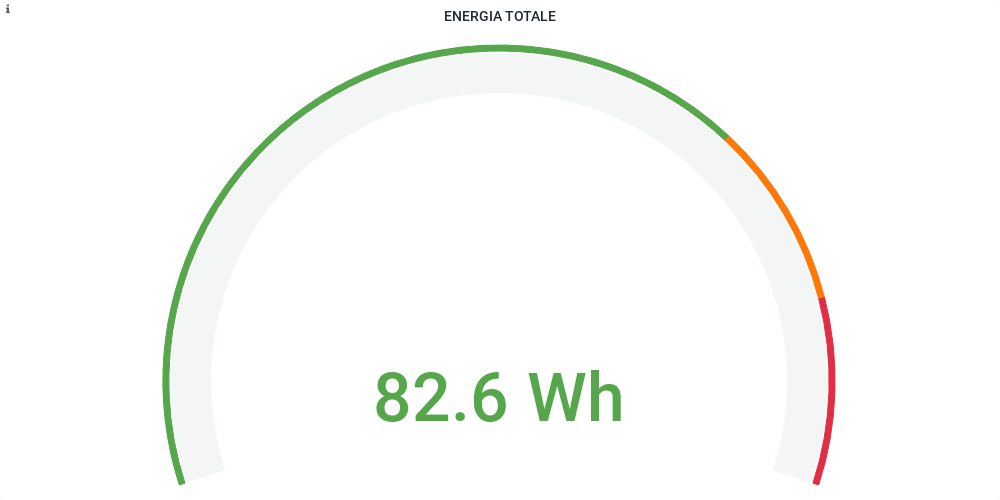
\includegraphics[scale=0.4, width=0.5\textwidth]{image43}
\end{figure}
\begin{flushleft}
L'energia media consumata rientra negli standard delle CPU moderne.
\end{flushleft}
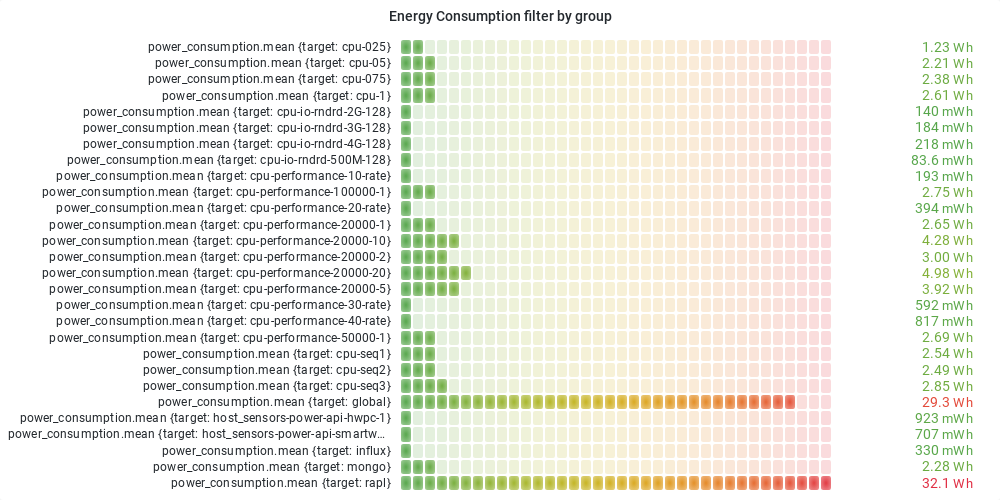
\includegraphics[scale=0.4]{image41}
\clearpage
\subsubsection{Analisi consumi energetici database}
\begin{flushleft}
{Vengono analizzati i consumi energetici dei database coinvolti nell'utilizzo di POWERAPI}
\end{flushleft}
\begin{figure}[h]
\caption{CONSUMI ENERGETICI DATABASE}
\centering
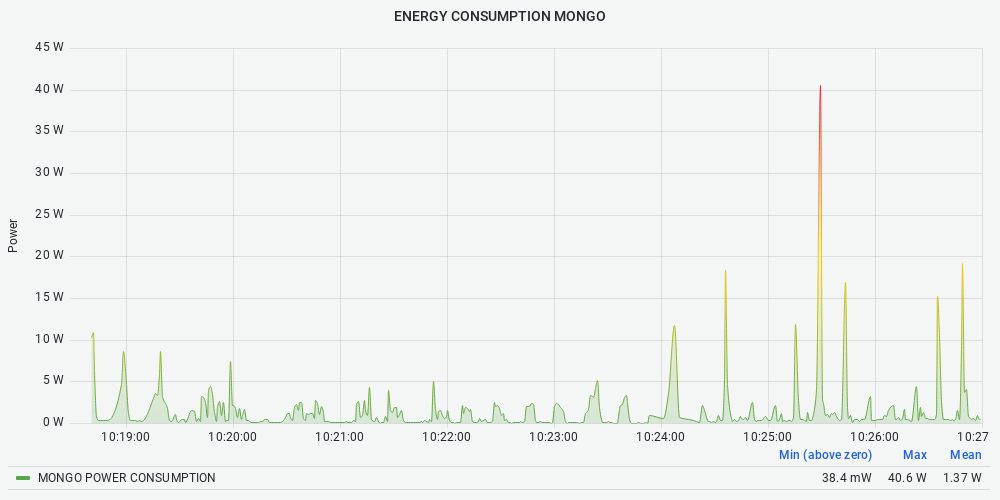
\includegraphics[scale=0.4]{image4}
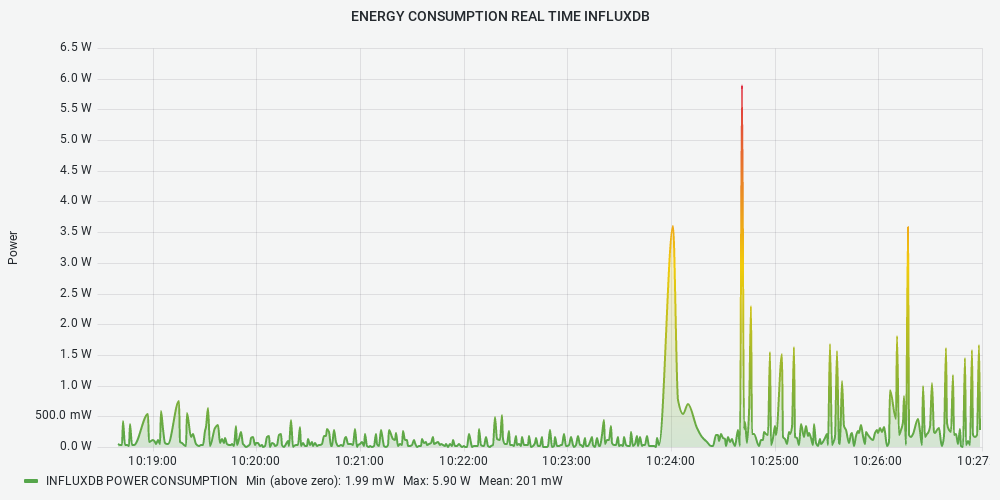
\includegraphics[scale=0.4]{image7}
\end{figure}

\clearpage
\section{Tests con sysbench}
\subsection{Sequential cpu test}
\begin{flushleft}
Vengono eseguite tre diverse run di sysbench cpu - rispettivamente con tre diverse tempistiche. Test base per verificare l'incremento dei consumi energetici all'incremento dei container docker in esecuzione.
\end{flushleft}
\begin{figure}[h]
\caption{SEQUENTIAL-CPU-TEST}
\centering
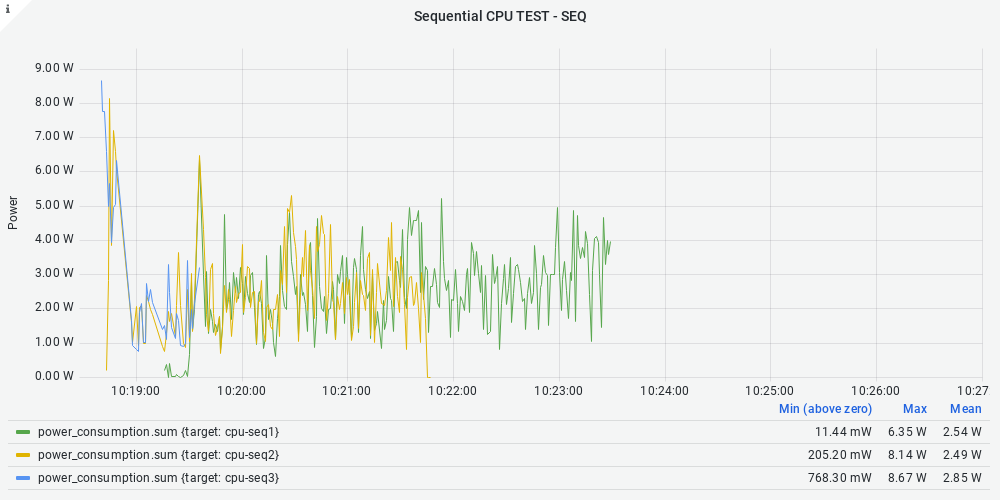
\includegraphics[scale=0.4]{image25}
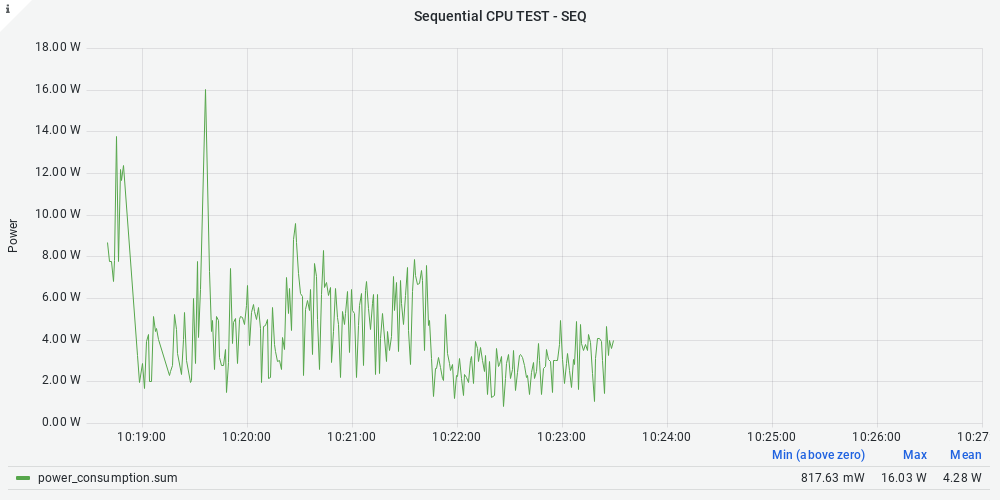
\includegraphics[scale=0.4]{image34}
\end{figure}

\clearpage
\subsection{Cpu-performance-n-rate}
\begin{flushleft}
Ogni container rappresenta una run sysbench variando il parametro rate.
\begin{center}
\textbf{N-rate : Tasso medio di transazioni.}
\end{center}
Si vede come all'incrementare del tasso medio di transazioni (RATE) incrementano i consumi energetici.
\end{flushleft}
\begin{figure}[h]
\caption{CPU-PERFORMANCE-N-RATE}
\centering
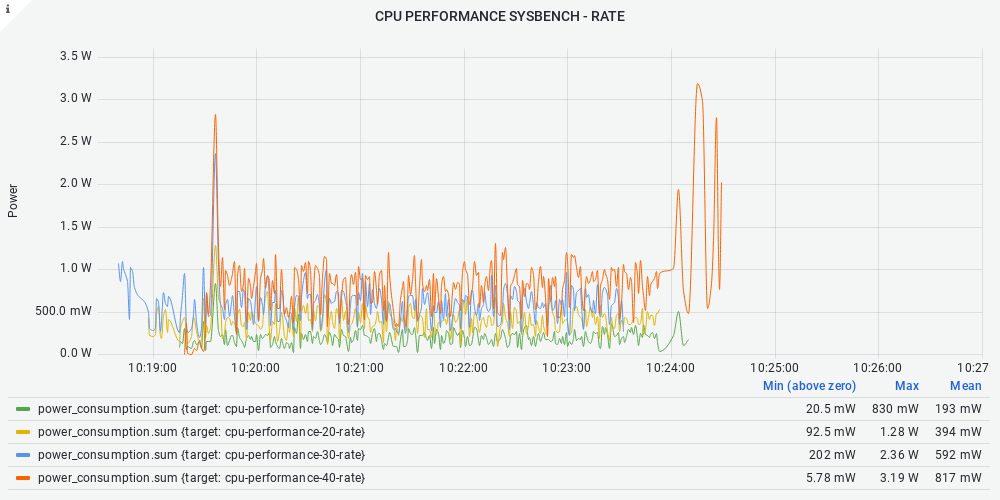
\includegraphics[scale=0.4]{image19}
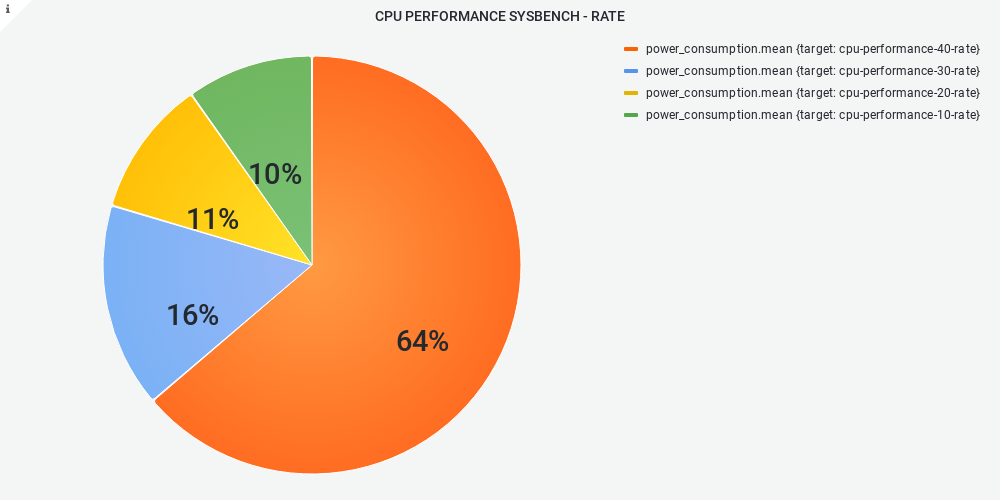
\includegraphics[scale=0.4]{image37}
\end{figure}
\clearpage
\subsection{Cpu-performance-P-N}
Il benchmark è configurato con il numero di thread simultanei e il numero massimo per verificare se è un numero primo.
\begin{flushleft}
\begin{itemize}
\item Ogni container rappresenta una run sysbench con questi parametri :
\begin{itemize}
\item P : cpu-max-prime
\item N : number of threads
\end{itemize}
\end{itemize}
\end{flushleft}
\begin{itemize}
\item  Variando il numero di threads. 
\begin{figure}[h]
\caption{CPU-PERFORMANCE-P-N (threads)}
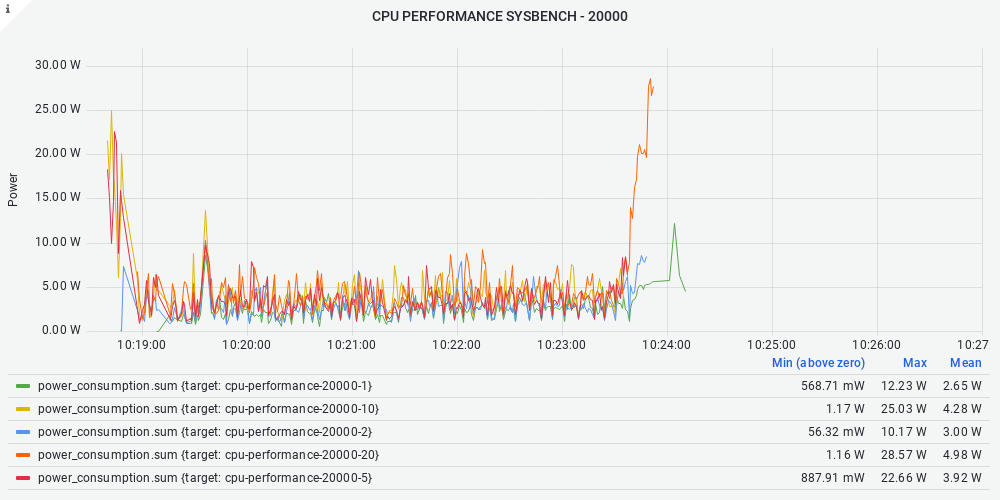
\includegraphics[scale=0.4]{image10}
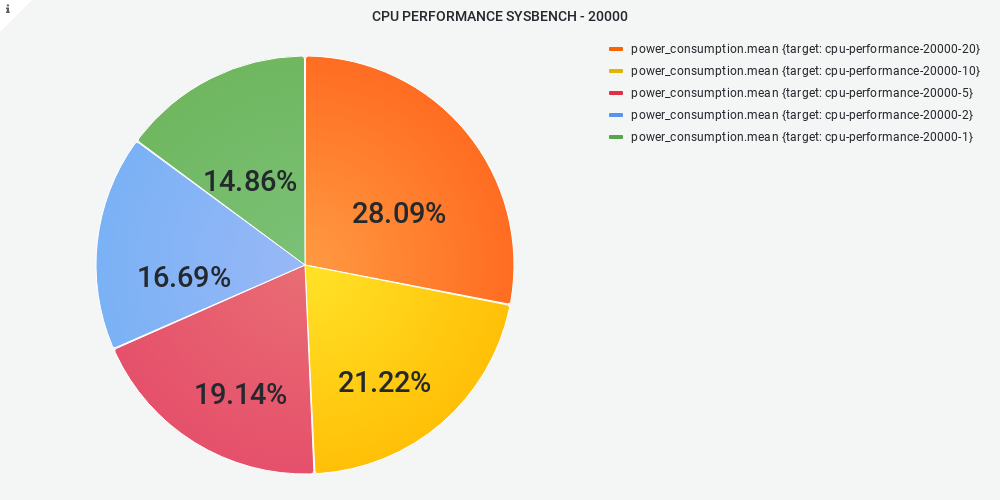
\includegraphics[scale=0.4]{image38}
\\ Si vede come all'incrementare del numero di threads coinvolti nel test, incrementano i consumi energetici.
\end{figure}
\clearpage
\item Variando cpu-max-prime.
\begin{figure}[h]
\caption{CPU-PERFORMANCE-P-N (cpu-max-prime)}
\begin{flushleft}
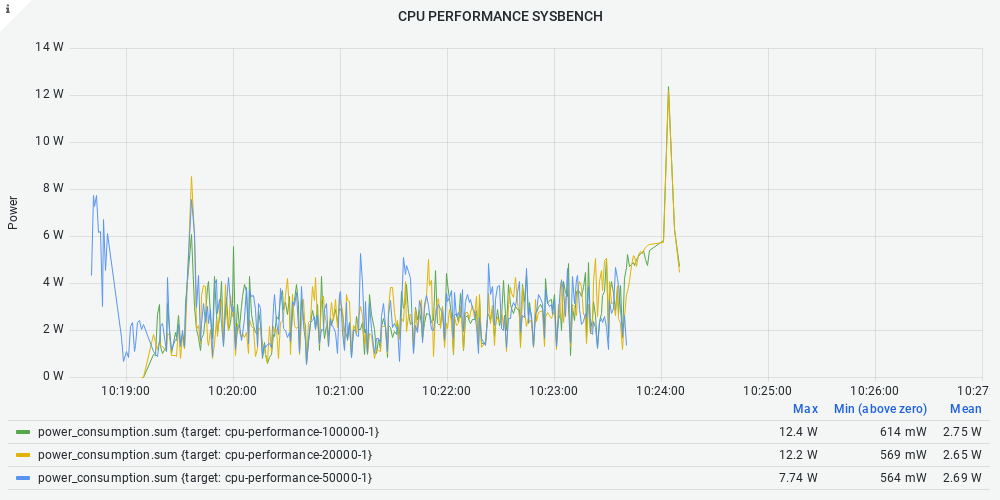
\includegraphics[scale=0.4]{image8}
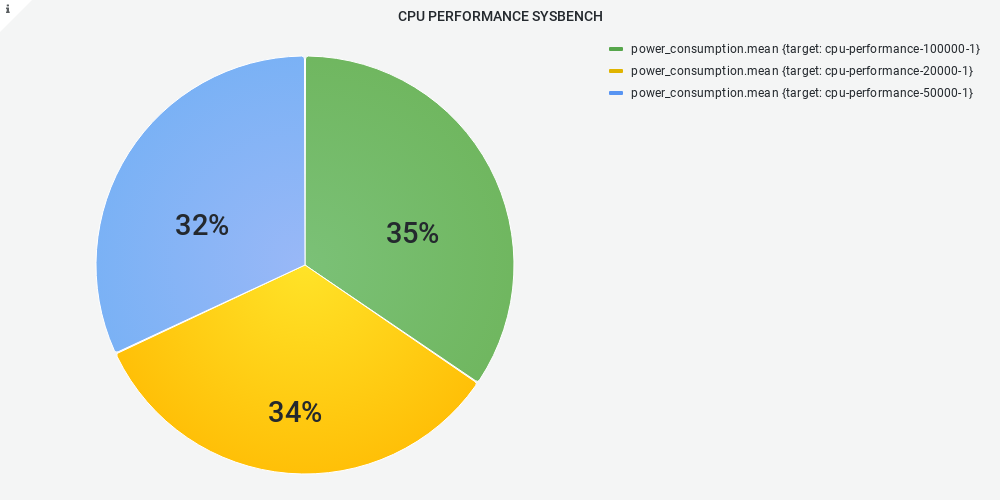
\includegraphics[scale=0.4]{image39}
\end{flushleft}
\end{figure}
\end{itemize}
\clearpage
\subsection{Cpu-performance cpus limit}
\begin{flushleft}
In questi test viene usato il comando '--cpu=x' che permette di limitare l'utilizzo della cpu.
Si vede come all'incrementare della cpu assegnata incrementano i consumi energetici.
\end{flushleft}
\begin{figure}[h]
\caption{CPU-PERFORMANCE-CPUS-LIMIT}
\centering
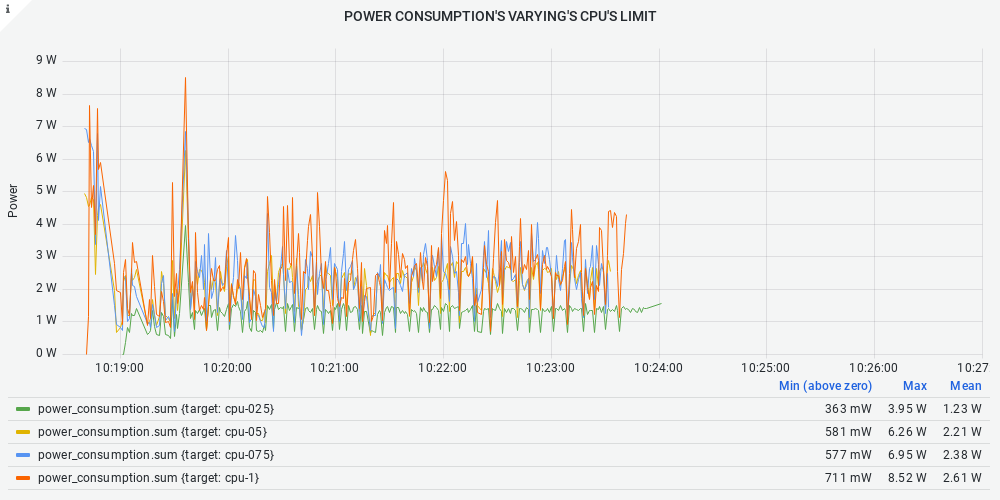
\includegraphics[scale=0.4]{image30}
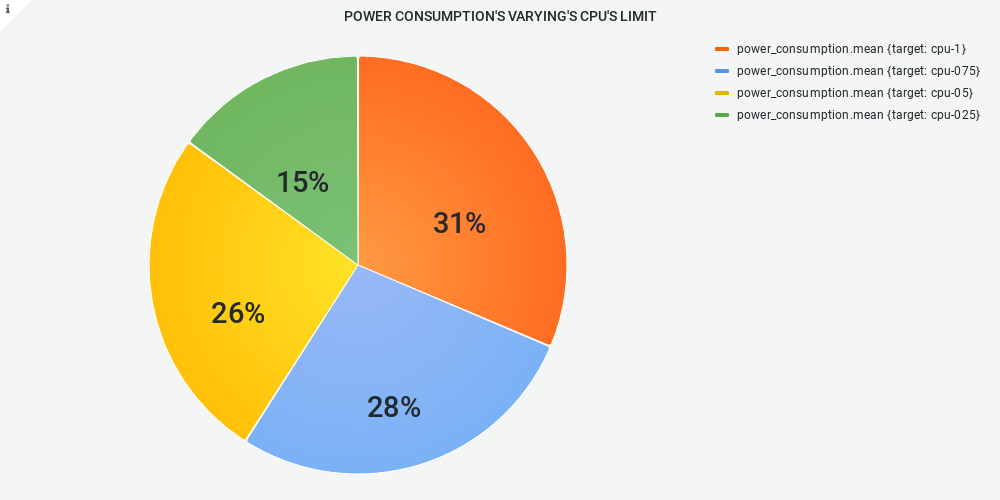
\includegraphics[scale=0.4]{image35}
\begin{flushleft}
{\ La schermata permette di vedere la percentuale di CPU assegnata ad ogni container : }
\end{flushleft}
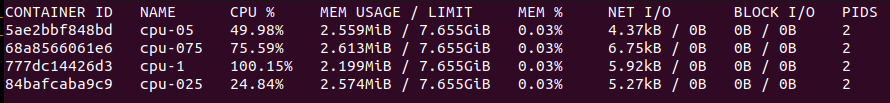
\includegraphics[scale=0.4]{cpus}

\end{figure}
\begin{flushleft}

\end{flushleft}
\clearpage
\subsection{Cpu-performance sysbench IO}
\begin{flushleft}
In queste run viene testato sysbench IO.
\begin{itemize}
\item S: --file-total-size (grandezza di 1 file)
\item N: --file-num (numero di file)
\end{itemize}
\end{flushleft}
\begin{flushleft}
Si vede come all'incrementare della dimensione dei file, incrementano i consumi energetici.
\end{flushleft}

\begin{figure}[h]
\caption{CPU-IO-RNDRD-S-N}
\centering
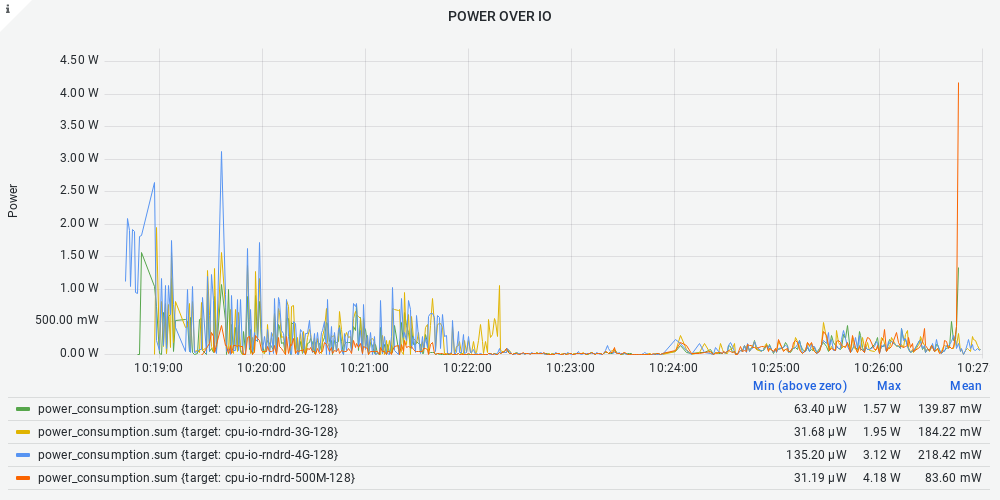
\includegraphics[scale=0.4]{image33}
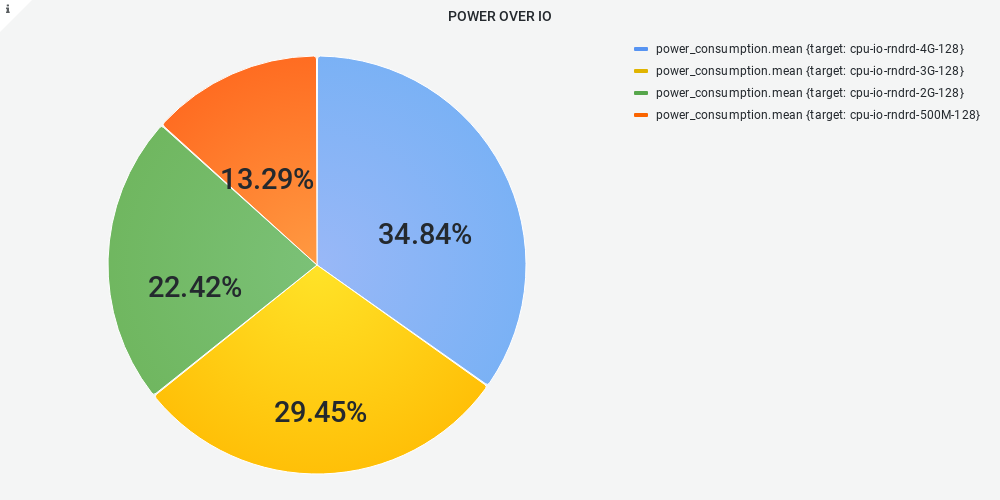
\includegraphics[scale=0.4]{image36}
\end{figure}
\ldots

\pagebreak
\listoffigures

\clearpage
\nocite{*}
\printbibliography


\end{document}

